
%----------------------------------------------------------------------------------------
%	PACKAGES AND OTHER DOCUMENT CONFIGURATIONS
%----------------------------------------------------------------------------------------

\documentclass[
11pt, % The default document font size, options: 10pt, 11pt, 12pt
english, % ngerman for German
singlespacing, % Single line spacing, alternatives: 
headsepline, % Uncomment to get a line under the header
oneside,
]{MastersDoctoralThesis} % The class file specifying the document structure
\usepackage[utf8]{inputenc} % Required for inputting international characters
\usepackage[T1]{fontenc} % Output font encoding for international characters
\usepackage{palatino} % Use the Palatino font by default
\usepackage[backend=bibtex,style=numeric,natbib=true]{biblatex} % Use the bibtex backend with the authoryear citation style (which resembles APA)
%\addbibresource{example.bib} % The filename of the bibliography


\addbibresource{references.bib} % The filename of the bibliography
\usepackage[autostyle=true]{csquotes} % Required to generate language-dependent quotes in the bibliography
\usepackage{algorithm}% http://ctan.org/pkg/algorithms
\usepackage{algpseudocode}% http://ctan.org/pkg/algorithmicx
\usepackage{amsmath}

%----------------------------------------------------------------------------------------
%	MARGIN SETTINGS
%----------------------------------------------------------------------------------------

\geometry{
	paper=a4paper, % Change to letterpaper for US letter
	inner=2.5cm, % Inner margin
	outer=3.8cm, % Outer margin
	bindingoffset=.5cm, % Binding offset
	top=1.5cm, % Top margin
	bottom=1.5cm, % Bottom margin
	%showframe, % Uncomment to show how the type block is set on the page
}

%----------------------------------------------------------------------------------------
%	THESIS INFORMATION
%----------------------------------------------------------------------------------------

\thesistitle{Thesis Title} % Your thesis title, this is used in the title and abstract, print it elsewhere with \ttitle
\supervisor{Vasilis Samoladas} % Your supervisor's name, this is used in the title page, print it elsewhere with \supname
\degree{Electrical and Computer Engineer} % Your degree name, this is used in the title page and abstract, print it elsewhere with \degreename
\author{Stefanos Stathatos} % Your name, this is used in the title page and abstract, print it elsewhere with \authorname

\subject{} % Your subject area, this is not currently used anywhere in the template, print it elsewhere with \subjectname
\keywords{} % Keywords for your thesis, this is not currently used anywhere in the template, print it elsewhere with \keywordnames
\university{\href{http://www.tuc.gr}{Technical University of Crete}} % Your university's name and URL, this is used in the title page and abstract, print it elsewhere with \univname
\department{\href{http://http://www.ece.tuc.gr/index.php?id=4101}{School of Electrical and Computer Engineering}} % Your department's name and URL, this is used in the title page and abstract, print it elsewhere with \deptname
\group{} % Your research group's name and URL, this is used in the title page, print it elsewhere with \groupname
\faculty{\href{http://www.tuc.gr}{Technical University of Crete}} % Your faculty's name and URL, this is used in the title page and abstract, print it elsewhere with \facname

\AtBeginDocument{
\hypersetup{pdftitle=\ttitle} % Set the PDF's title to your title
\hypersetup{pdfauthor=\authorname} % Set the PDF's author to your name
\hypersetup{pdfkeywords=\keywordnames} % Set the PDF's keywords to your keywords
}

\begin{document}

%\frontmatter % Use roman page numbering style (i, ii, iii, iv...) for the pre-content pages

\pagestyle{plain} % Default to the plain heading style until the thesis style is called for the body content



%----------------------------------------------------------------------------------------
%	TITLE PAGE
%----------------------------------------------------------------------------------------

\begin{titlepage}
\begin{center}

\vspace*{.06\textheight}
{\scshape\LARGE \univname\par}\vspace{1.5cm} % University name
\textsc{\Large Thesis}\\[0.5cm] % Thesis type

\HRule \\[0.4cm] % Horizontal line
{\huge \bfseries \ttitle\par}\vspace{0.4cm} % Thesis title
\HRule \\[1.5cm] % Horizontal line
 
\emph{Author:}\\
{\authorname} % Author name - remove the \href bracket to remove the link
\vspace{20pt}

\emph{Committee:} \\
{Associate Professor} {\supname} (Supervisor)\\
{Associate Professor} Minos Garofalakis\\
{Associate Professor} Kostas Petrakis\\
\vspace{20pt}
\vfill

\large \textit{A thesis submitted in fulfillment of the requirements\\ for the degree of \degreename}\\[0.3cm] % University requirement text
\textit{in the}\\[0.4cm]
\deptname\\\univname\\[2cm] % Research group name and department name
 
\vfill

{\large \today}\\[4cm] % Date
%\includegraphics{Logo} % University/department logo - uncomment to place it
 
\vfill
\end{center}
\end{titlepage}


%----------------------------------------------------------------------------------------
%	ABSTRACT PAGE
%----------------------------------------------------------------------------------------

\begin{abstract}
\addchaptertocentry{\abstractname} % Add the abstract to the table of contents
The Thesis Abstract is written here (and usually kept to just this page). The page is kept centered vertically so can expand into the blank space above the title too\ldots
\end{abstract}

%----------------------------------------------------------------------------------------
%	ACKNOWLEDGEMENTS
%----------------------------------------------------------------------------------------

\begin{acknowledgements}
\addchaptertocentry{\acknowledgementname} % Add the acknowledgements to the table of contents
The acknowledgments and the people to thank go here, don't forget to include your project advisor\ldots
\end{acknowledgements}

%----------------------------------------------------------------------------------------
%	LIST OF CONTENTS/FIGURES/TABLES PAGES
%----------------------------------------------------------------------------------------

\tableofcontents % Prints the main table of contents

\listoffigures % Prints the list of figures


%----------------------------------------------------------------------------------------
%	THESIS CONTENT - CHAPTERS
%----------------------------------------------------------------------------------------

\mainmatter % Begin numeric (1,2,3...) page numbering

\pagestyle{thesis} % Return the page headers back to the "thesis" style

% Introduction

\chapter{Introduction} % Main chapter title

\section{Overview}
The World Wide Web has been central to the development of the Information Age and is the primary tool billions of people use to interact on the Internet. The huge growth of Web in the last years has lead to the demand for specialized applications, which operate in different devices, are secure and guarantee the constant provision of services to the user, under any circumstances. The software development process can be delivered at the same time by multiple stakeholders, which are located in different areas of the world, studying and working on the same code. Meanwhile, the time-consuming stages of production necessitate the proper software design, with the purpose of minimizing the possibility of large design flaws or discovering them in early stages. \par 
	The model driven software development is a design technique which is based in model utilization and assists in the creation of software, which is extensible, reusable and comprehensible by different stakeholders. It contributes in the development of isolated modules with seperated responsibilities. Hence, this design approach is an ideal solution for creating carefully developed, well tested software, which can be upgraded at any moment. \par 
	Another challenge of the time we are in, is the daily touch with large amounts of complex data, which one must constantly study in order to draw conclusions and make decisions. Because of the way the human brain processes information, using charts or graphs to visualize data is easier than poring over spreadsheets or reports. Data visualization is the presentation of data in a pictorial or graphical format. It enables decision makers to see analytics presented visually, so they can grasp difficult concepts or identify new patterns. \par
	In this thesis, we developed a data visualization framework, which follows the principles of model driven programming. The hierarchical data format is utilized for storing complex multidimensional datasets. The framework implements a method to present visually the datasets to the users, which enables easy understanding, conclusion extraction and decision making. \par 
	The framework consists of modules which contain generic code and are configurable by other modules. The framework's functionality is expanded, either through the development of a new independent module or via the growth of an existing one. The model driven approach enables the system's adaptability based on the designer's requirements. \par 
	The framework presentation is implemented through the creation of a web application, which operates as a data visualization tool, for networks of users working on the same projects. The projects contain datasets, posts and plots, which are visible by all project members. The plots are used as a graphical representation of the datasets. \par
	Among other things, the user may interact with the datasets through the diagrams. We implemented a zoom functionality, which enables  switching between the detail levels of the visualized datasets. While the abstract representation of large datasets is possible, the display of small details is also available. The retrieval of sampled chunks of HDF files makes the zoom functionality efficient.   \par 
	The framework, as well as the application, are mainly developed in the javascript programming language. Especially the front end tier was developed exclusively in pure javascript, without the usage of a large framework. The front end follows the principles of the single page application design approach.


%I terastia anaptuksi tou exei odigisei stin anagki gia dimiourgia ekseidikeumenwn efarmogwn, oi opoies leitourgoun se polles diaforetikes suskeues, einai asfaleis kai egguontai tin sunexi paroxi upiresiwn sto xristi upo opoiesdipote sunthikes. I idia i anaptuksi efarmogwn pleon mporei na ginetai apo apo pollous stakeholders tautoxrona, oi opoioi vriskontai se diaforetika simeia tou kosmou kai meletoun k epemvainoun se koino kwdika. Parallila, ta xronovora stadia paragwgis kathistoun megali proteraiotita ton swsto sxediasmo tou logismikou, etsi wste na elaxistopoiithoun i na anakalufthoun sta prwta stadia, megala sxediastika flaws. \par
%	To model-driven software development einai mia sxediastiki texniki i opoia vasizetai stin anaptuksi montelwn, kai voithaei stin paragwgi logismikou to opoio einai epektasimo, reusable kai eukola katanoito apo diaforetikous stakeholders. Suneisferei stin dimiourgia modules kwdika isolated metaksu tous kai me ksexwrista responsibilities. Epomenws, to sugekrimeno sxediastiko approach einai idaniki lusi gia tin dimiourgia prosektika grammenou tested logismikou pou mporei ana pasa stigmi na anavathmistei. \par
%	Ena allo xaraktiristiko tis epoxis pou dianioume einai i kathimerini epafi me large amounts of complex data, ta opoia prepei kaneis na meletaei wste na vgazei sumperasmata kai na pairnei apofaseis. Because of the way the human brain processes information, using charts or graphs to visualize data is easier than poring over spreadsheets or reports. Data visualization is the presentation of data in a pictorial or graphical format. It enables decision makers to see analytics presented visually, so they can grasp difficult concepts or identify new patterns. \par
%
%	In this thesis, anaptusoume ena data visualization framework, to opoio akolouthei tis arxes tou montelostrafous programmatismou. Xrisimopoiei to hierachical data format, gia na apothikeusei complex multidimentional datasets. To framework ulopoiei mia methodo dataset visualization stous xristes, to opoio epitrepei tin eukoli katanoisi, eksagwgi sumperasmatwn kai decision making. \par 
%	Gia tin anaptuksi tou, dimiourgithikan modules ta opoia periexoun generic kwdika kai einai parametropoiisima apo alla modules. Auto exei ws apotelesma tin paragwgi reusable kai extensible modules ta opoia sundiazontai metaksu tous gia tin dimiourgia tou framework. I parousiasi tou framework ginetai mesw tis dimiourgias mias web efarmogis, i opoia leitourgei ws ena data visualization tool gia diktua apo users oi opoioi ergazontai se koina projects. To framework, opws kai i efarmogi, ulopoiithikan sto megalutero vathmo se javascript.
\section{Outline}
Chapter ~\ref{chapter2_bg} provides the necessary theoretical background used throughout this thesis, including model driven software development, data access object, access control list and RESTful web service. An overview of the related work and technologies used is presented in chapter ~\ref{chapter3_rw}. The proposed detailed framework architecture is described in chapter ~\ref{chapter4_d}. In chapter~\ref{chapter5_i} we discuss the framework and application implementation as well as the technologies we utilized. Next, we evaluate the framework performance in chapter~\ref{chapter6_pe}. Finally, the conclusion and future work are presented in chapter~\ref{chapter7_cf}. 
% Background

\chapter{Background} % Main chapter title

\label{chapter2_bg}
This chapter presents some background for the content of this thesis. We introduce theoretical concepts, such as model driven software development, data access object, access control list, HTTP protocol and RESTful web services.

\section{Models and Model Driven Software Development}
\label{mdsd}
Software development is a complex and difficult task that requires the investment of significant resources and carries a major risk of failure. According to its proponents, model-driven (MD) software development approaches are improving the way we build software. Model-driven approaches hypothetically increase developer productivity, decrease the cost (in time and money) of software construction, improve software reusability, and make software more maintainable. Likewise, model-driven techniques promise to contribute to the early detection of defects such as design flaws, omissions, and misunderstandings between clients and developers. \par
	If a model is a representation of a system, then in some sense, programming in any language involves some kind of model. Whether we explicitly create artifacts we call models—especially conceptual models—or whether we implicitly map between our internal mental models of the world and the systems we produce, we are nevertheless involved in a modeling process as we construct software. And so MD is more about raising the level of abstraction of our programming models rather than introducing models into the process in the first place. Models  help software engineers communicate more effectively with the many stakeholders who need to participate in the software development process. Improved communication leads to increased understanding, more reasonable expectations, and a better overall work product. Models also let programmers visualize the finished product without requiring its full construction first. By examining the model we can discover design flaws that are far less expensive to resolve up-front rather than after construction has begun (or worse, been completed).\par
	Model-driven software development~\cite{liddle2011model} is a software design approach for the development of software systems. It provides a set of guidelines for the structuring of specifications, which are expressed as models. Model-driven architecture (MDA) is a kind of domain engineering, and supports model-driven engineering of software systems.\par
	The three primary goals of MDA are portability, interoperability, and reusability, and the key abstraction for delivering on these goals is architectural separation of concerns. Architectural separation of concerns is a design principle for separating a computer program into distinct sections, such that each section addresses a separate concern. A concern is a set of information that affects the code of a computer program. When concerns are well-separated, individual sections can be reused, as well as developed and updated independently. Of special value is the ability to later improve or modify one section of code without having to know the details of other sections, and without having to make corresponding changes to those sections. In this way, architectural separation of concerns accomplishes the primary goals of MDA. Thus, developing generic, customizable, independent modules with seperated responsibilities implements the model driven software development approach.
  


\section{Data Access Object}
\label{dao}
In computer software, a data access object (DAO)~\cite{DAO} is an object that provides an abstract interface to some type of database or other persistence mechanism. By mapping application calls to the persistence layer, the DAO provides some specific data operations without exposing details of the database. This isolation supports the single responsibility principle. It separates what data access the application needs, in terms of domain-specific objects and data types (the public interface of the DAO), from how these needs can be satisfied with a specific DBMS or database schema. Because the interface exposed by the DAO to clients does not change when the underlying data source implementation changes, this pattern allows the DAO to adapt to different storage schemes without affecting its clients or business components. Essentially, the DAO acts as an adaptor between the component and the data source.\par 
	The advantage of using data access objects is the relatively simple and rigorous separation between two important parts of an application that can but should not know anything of each other, and which can be expected to evolve frequently and independently. Changing business logic can rely on the same DAO interface, while changes to persistence logic do not affect DAO clients as long as the interface remains correctly implemented. All details of storage are hidden from the rest of the application. Thus, possible changes to the persistence mechanism can be implemented by just modifying one DAO implementation while the rest of the application isn't affected. DAOs act as an intermediary between the application and the database. They move data back and forth between objects and database records.

\section{Access Control List}
\label{acl}
An Access Control List (ACL)~\cite{shirey2007internet} is a mechanism that implements access control for a system resource by enumerating the system 	entities that are permitted to access the resource and stating, either implicitly or explicitly, the access modes granted to each entity. A filesystem ACL is a data structure (usually a table) containing entries that specify individual user or group rights to specific system objects such as programs, processes, or files. \par
	In computing, permission is defined as the delegation of authority over a computer system. A permission allows a user to perform an action. Examples of various privileges include the ability to create a file in a directory, or to read or delete a file, access a device, or have read or write permission to a socket for communicating over the Internet. The permissions to perform certain operations are assigned to specific roles. Members or administrators (or other system users) are assigned particular roles, and through those role assignments acquire the computer permissions to perform particular computer-system functions.

\section{HTTP}
The Hypertext Transfer Protocol (HTTP)~\cite{fielding2006hypertext} is an application-level protocol for distributed, collaborative, hypermedia information systems. HTTP has been in use by the World-Wide Web global information initiative since 1990. HTTP functions as a request–response protocol in the client–server computing model. A web browser, for example, may be the client and an application running on a computer hosting a website, may be the server. The client submits an HTTP request message to the server. The server, which provides resources such as HTML files and other content or performs other functions on behalf of the client, returns a response message to the client. The response contains completion status information about the request and may also contain requested content in its message body. HTTP resources are identified and located on the network by Uniform Resource Locators (URL), using the Uniform Resource Identifiers (URI) schemes http and https. URI and hyperlinks in HTML documents form inter-linked hypertext documents.




\subsection{HTTP session}
An HTTP session is a sequence of network request-response transactions. An HTTP client initiates a request by establishing a Transmission Control Protocol (TCP) connection to a particular port on a server. An HTTP server listening on that port waits for a client's request message. Upon receiving the request, the server sends back a status line, such as "HTTP/1.1 200 OK", and a message of its own. The body of this message is typically the requested resource, although an error message or other information may also be returned.




\subsection{Request methods}
HTTP defines methods to indicate the desired action to be performed on the identified resource. What this resource represents, whether pre-existing data or data that is generated dynamically, depends on the implementation of the server. The most common methods which are used in this thesis are presented below.

\paragraph{GET}
The GET method requests a representation of the specified resource. Requests using GET should only retrieve data and should have no other effect. The W3C has published guidance principles on this distinction, saying, "Web application design should be informed by the above principles but also by the relevant limitations".

\paragraph{POST}
The POST method requests that the server accepts the entity enclosed in the request as a new subordinate of the web resource identified by the URI. The data POSTed might be, for example, an annotation for existing resources; a message for a bulletin board, newsgroup, mailing list, or comment thread; a block of data that is the result of submitting a web form to a data-handling process; or an item to add to a database.

\paragraph{PUT}
The PUT method requests that the enclosed entity be stored under the supplied URI. If the URI refers to an already existing resource, it is modified; if the URI does not point to an existing resource, then the server can create the resource with that URI.

\paragraph{DELETE}
The DELETE method deletes the specified resource.




\subsection{Status Codes}
In HTTP/1.0 and since, the first line of the HTTP response is called the status line and includes a numeric status code (such as "404") and a textual reason phrase (such as "Not Found"). The way the user agent handles the response primarily depends on the code and secondarily on the other response header fields. Custom status codes can be used since, if the user agent encounters a code it does not recognize, it can use the first digit of the code to determine the general class of the response. HTTP status code is primarily divided into five groups for better explanation of request and responses between client and server, and are presented below. 

\paragraph{1xx Informational responses}
An informational response indicates that the request was received and understood. It is issued on a provisional basis while request processing continues. It alerts the client to wait for a final response. The message consists only of the status line and optional header fields, and is terminated by an empty line.

\paragraph{2xx Success}
This class of status codes indicates the action requested by the client was received, understood, accepted, and processed successfully.

\paragraph{3xx Redirection}
This class of status code indicates the client must take additional action to complete the request. Many of these status codes are used in URL redirection.
A user agent may carry out the additional action with no user interaction only if the method used in the second request is GET or HEAD. A user agent may automatically redirect a request. A user agent should detect and intervene to prevent cyclical redirects.

\paragraph{4xx Client errors}
This class of status code is intended for situations in which the client seems to have errored. Except when responding to a HEAD request, the server should include an entity containing an explanation of the error situation, and whether it is a temporary or permanent condition. These status codes are applicable to any request method. User agents should display any included entity to the user.

\paragraph{5xx Server errors}
The server failed to fulfill an apparently valid request: response status codes beginning with the digit "5" indicate cases in which the server is aware that it has encountered an error or is otherwise incapable of performing the request. Except when responding to a HEAD request, the server should include an entity containing an explanation of the error situation, and indicate whether it is a temporary or permanent condition. Likewise, user agents should display any included entity to the user. These response codes are applicable to any request method.




\section{Representational State Transfer}
\label{rest}
Representational state transfer (REST)~\cite{w3c2004web} or RESTful web services is a way of providing interoperability between computer systems on the Internet. REST-compliant Web services allow requesting systems to access and manipulate textual representations of Web resources using a uniform and predefined set of stateless operations.  In a RESTful Web service, requests made to a resource's URI will elicit a response that may be in XML, HTML, JSON or some other defined format. The response may confirm that some alteration has been made to the stored resource, and it may provide hypertext links to other related resources or collections of resources.\par  		The term is intended to evoke an image of how a well-designed Web application behaves: it is a network of Web resources (a virtual state-machine) where the user progresses through the application by selecting links, such as /user/tom, and operations such as GET or DELETE (state transitions), resulting in the next resource (representing the next state of the application) being transferred to the user. There are six guiding constraints that define a RESTful system. These constraints restrict the ways that the server may process and respond to client requests so that, by operating within these constraints, the service gains desirable non-functional properties, such as performance, scalability, simplicity, modifiability, visibility, portability, and reliability. If a service violates any of the required constraints, it cannot be considered RESTful. The formal REST constraints are represented below.

\subsection{Client-server architecture}
The first constraints added to our hybrid style are those of the client-server architectural style. Separation of concerns is the principle behind the client-server constraints. By separating the user interface concerns from the data storage concerns, we improve the portability of the user interface across multiple platforms and improve scalability by simplifying the server components. Perhaps most significant to the Web, however, is that the separation allows the components to evolve independently, thus supporting the Internet-scale requirement of multiple organizational domains.

\paragraph{Statelessness}
The client–server communication is constrained by no client context being stored on the server between requests. Each request from any client contains all the information necessary to service the request, and session state is held in the client. The session state can be transferred by the server to another service such as a database to maintain a persistent state for a period and allow authentication. The client begins sending requests when it is ready to make the transition to a new state. While one or more requests are outstanding, the client is considered to be in transition. The representation of each application state contains links that may be used the next time the client chooses to initiate a new state-transition.

\paragraph{Cacheability}
As on the World Wide Web, clients and intermediaries can cache responses. Responses must therefore, implicitly or explicitly, define themselves as cacheable or not to prevent clients from reusing stale or inappropriate data in response to further requests. Well-managed caching partially or completely eliminates some client–server interactions, further improving scalability and performance.

\paragraph{Layered system}
A client cannot ordinarily tell whether it is connected directly to the end server, or to an intermediary along the way. Intermediary servers may improve system scalability by enabling load balancing and by providing shared caches. They may also enforce security policies.

\paragraph{Uniform interface}
The uniform interface constraint is fundamental to the design of any REST service. It simplifies and decouples the architecture, which enables each part to evolve independently.





\section{Application Programming Interface}
In computer programming, an Application Programming Interface (API) is a set of subroutine definitions, protocols, and tools for building application software. In general terms, it is a set of clearly defined methods of communication between various software components. A good API makes it easier to develop a computer program by providing all the building blocks, which are then put together by the programmer. An API may be for a web-based system, operating system, database system, computer hardware or software library. An API specification can take many forms, but often includes specifications for routines, data structures, object classes, variables or remote calls. API uses are listed below.

\paragraph{Libraries and Frameworks}
An API is usually related to a software library. The API describes and prescribes the expected behavior (a specification) while the library is an actual implementation of this set of rules. A single API can have multiple implementations (or none, being abstract) in the form of different libraries that share the same programming interface. The separation of the API from its implementation can allow programs written in one language to use a library written in another. 

\paragraph{Operating systems}
An API can specify the interface between an application and the operating system. POSIX, for example, specifies a set of common APIs that aim to enable an application written for a POSIX conformant operating system to be compiled for another POSIX conformant operating system.

\paragraph{Remote APIs}
Remote APIs allow developers to manipulate remote resources through protocols, specific standards for communication that allow different technologies to work together, regardless of language or platform.


\paragraph{WEB APIs}
Web APIs are the defined interfaces through which interactions happen between an enterprise and applications that use its assets. An API approach is an architectural approach that revolves around providing programmable interfaces to a set of services to different applications serving different types of consumers.When used in the context of web development, an API is typically defined as a set of Hypertext Transfer Protocol (HTTP) request messages, along with a definition of the structure of response messages, which is usually in an Extensible Markup Language (XML) or JavaScript Object Notation (JSON) format.

\section{Three-tier Architecture}
\label{3tierarch}
\begin{figure}
	\centerline{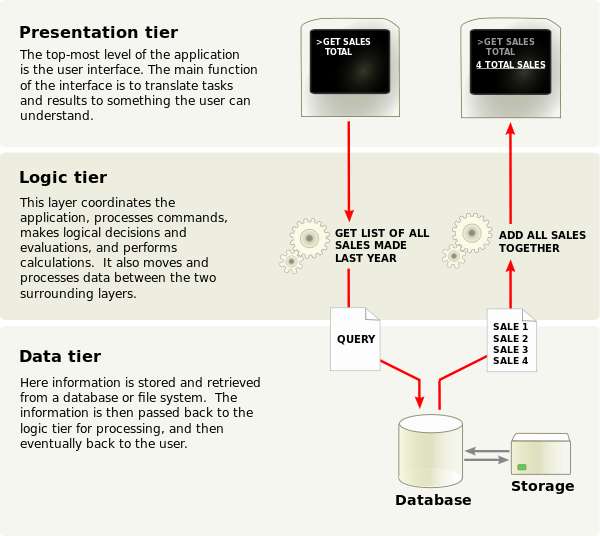
\includegraphics[scale=0.5]{3tier.png}}
	\caption{Three-tier Architecture}
	\label{3tier}
\end{figure}

Three-tier architecture~\cite{ramirez2000three} is a client–server software architecture pattern in which the user interface (presentation), functional process logic ("business rules"), computer data storage and data access are developed and maintained as independent modules, most often on separate platforms. Apart from the usual advantages of modular software with well-defined interfaces, the three-tier architecture is intended to allow any of the three tiers to be upgraded or replaced independently in response to changes in requirements or technology. An image of a three-tier architecture can be seen in figure~\ref{3tier}. The three layers are presented below.

\paragraph{Presentation tier}
This is the topmost level of the application. The presentation tier displays information related to such services as browsing merchandise, purchasing and shopping cart contents. It communicates with other tiers by which it puts out the results to the browser/client tier and all other tiers in the network. In simple terms, it is a layer which users can access directly (such as a web page, or an operating system's GUI).

\paragraph{Logic tier}
The logical tier is pulled out from the presentation tier and, as its own layer, it controls an application’s functionality by performing detailed processing.

\paragraph{Data tier}
The data tier includes the data persistence mechanisms (database servers, file shares, etc.) and the data access layer that encapsulates the persistence mechanisms and exposes the data. The data access layer should provide an API to the application tier that exposes methods of managing the stored data without exposing or creating dependencies on the data storage mechanisms. Avoiding dependencies on the storage mechanisms allows for updates or changes without the application tier clients being affected by or even aware of the change.




\section{Single Page Application}
\label{spa}
\begin{figure}
	\centerline{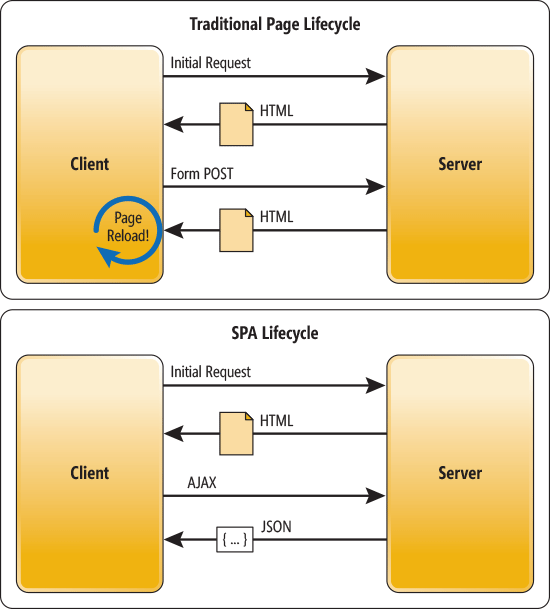
\includegraphics[scale=0.4]{spa.png}}
	\caption{Traditional page lifecycle vs Single Page Application Lifecycle}
	\label{spa}
\end{figure}
A single-page application (SPA)~\cite{mikowski2013single} is a web application or web site that fits on a single web page with the goal of providing a user experience similar to that of a desktop application. In a SPA, either all necessary code – HTML, JavaScript, and CSS – is retrieved with a single page load, or the appropriate resources are dynamically loaded and added to the page as necessary, usually in response to user actions. The page does not reload at any point in the process, nor does control transfer to another page, although the location hash or the HTML5 History API can be used to provide the perception and navigability of separate logical pages in the application. Interaction with the single page application often involves dynamic communication with the web server behind the scenes.\par
	There are various techniques available that enable the browser to retain a single page even when the application requires server communication. The most prominent technique currently being used is Ajax. Ajax is a set of Web development techniques using many Web technologies on the client side to create asynchronous Web applications. With Ajax, Web applications can send data to and retrieve from a server asynchronously (in the background) without interfering with the display and behavior of the existing page. By decoupling the data interchange layer from the presentation layer, Ajax allows for Web pages, and by extension Web applications, to change content dynamically without the need to reload the entire page. The difference between the traditional page and the SPA lifecycle can be seen in figure~\ref{spa}. In practice, modern implementations commonly substitute JSON for XML due to the advantages of being native to JavaScript.



\section{Hierarchical Data Format}
\label{hdf}
\begin{figure}
	\centerline{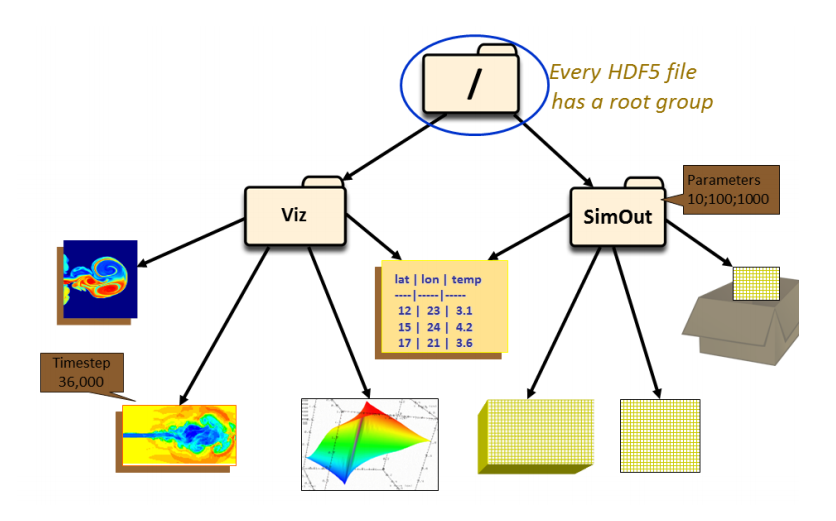
\includegraphics[scale=0.4]{hdf.png}}
	\caption{The contents of an HDF file}
	\label{hdf}
\end{figure}
\begin{figure}
	\centerline{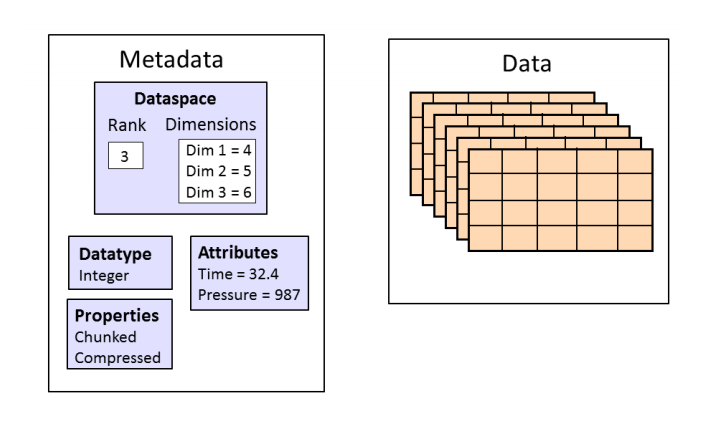
\includegraphics[scale=0.5]{dset.png}}
	\caption{The general structure of a dataset}
	\label{dset}
\end{figure}
Hierarchical Data Format (HDF))~\cite{hdf2014hierarchical} is a set of file formats (HDF4, HDF5) designed to store and organize large amounts of data. Many HDF adopters have very large datasets, very fast access requirements, or very complex datasets. Others turn to HDF because it allows them to easily share data across a wide variety of computational platforms using applications written in different programming languages.\par
	HDF allows hierarchical data objects to be expressed in a very natural manner, in contrast to the tables of a relational database.  Whereas relational databases support tables, HDF supports n-dimensional datasets and each element in the dataset may itself be a complex object. Relational databases offer excellent support for queries based on field matching, but are not well-suited for sequentially processing all records in the database or for subsetting the data based on coordinate-style lookup. The contents of an HDF file can be seen in figure~\ref{hdf}.\par
	HDF5 consists of a File Format for storing HDF5 data, a Data Model for logically organizing and accessing HDF5 data from an application, and the Software (libraries, language interfaces, and tools) for working with this format. The data model is described below.
\subsection{Data Model}
The HDF Data Model, also known as the HDF5 Abstract (or Logical) Data Model consists of the building blocks for data organization and specification in HDF5. An HDF5 file (an object in itself) can be thought of as a container (or group) that holds a variety of heterogeneous data objects (or datasets). The datasets can be most anything: images, tables, graphs, or even documents, such as PDF or Excel. The two primary objects in the HDF5 Data Model are described below.

\paragraph{Groups}
HDF5 groups (and links) organize data objects. Every HDF5 file contains a root group that can contain other groups or be linked to objects in other files. Working with groups and group members is similar in many ways to working with directories and files in UNIX. As with UNIX directories and files, objects in an HDF5 file are often described by giving their full (or absolute) path names.

\paragraph{Datasets}
HDF5 datasets organize and contain the “raw” data values. A dataset consists of metadata that describes the data, in addition to the data itself. Datatypes, dataspaces, properties and (optional) attributes are HDF5 objects that describe a dataset. The datatype describes the individual data elements. The general structure of a dataset can be seen in figure~\ref{dset}.













% Related Work

\chapter{Related Work and Technologies Used} % Main chapter title

\label{chapter3_rw}
This chapter contains the related work and the technologies used throughout this thesis. Initially, technologies that make use of functionalities similar with the content of our framework, are described. Following, we emphasize on the technologies we used throughout the development of our system.

\section{Related Work}

\subsection{Plotly}
Plotly is a popular public data visualization cloud service provider. Plotly provides community, professional and enterprise data storage, visualization and analytics services to the user.  Excel, CSV and XML data formats are used to upload the data to its cloud servers.  It also offers online graphing, analytics, and statistics tools for individuals and collaboration, as well as scientific graphing libraries for Python, R, MATLAB, Perl, Julia, Arduino, and REST. Although Plotly provides a large set of functionalities, it does not offer a way to visualize large multidimensional datasets.

\subsection{Loopback}
Loopback is a highly-extensible, open-source Node.js framework which assimilates the best practices of model driven software development. Loopback simplifies and speeds up REST API development. It consists of a library of Node.js modules for connecting web and mobile apps to data sources such as databases and REST APIs, a command line tool, and client-SDKs. A loopback application has three components: models that represent business data and behavior, data sources and connectors, and mobile clients. An application interacts with data sources through the loopback model API, available locally within Node, remotely over REST, and via native client APIs for iOS, Android, and HTML5. Using the API, apps can query databases, store data, upload files, send emails, create push notifications, register users, and perform other actions provided by data sources.
	Loopback is implemented with many of the technologies we use in this thesis. It uses MDSD as a general practice, data access objects for the communication between database and the server, access control list for  authorization and is written in Node.js.

\section{Technologies Used}

\subsection{HTML5}
HTML5~\cite{pilgrim2010html5} is a markup language used for structuring and presenting content on the World Wide Web. It is the fifth and current major version of the HTML standard.\par
It was published in October 2014 by the World Wide Web Consortium (W3C) to improve the language with support for the latest multimedia, while keeping it both easily readable by humans and consistently understood by computers and devices such as web browsers, parsers, etc. HTML5 is intended to subsume not only HTML 4, but also XHTML 1 and DOM Level 2 HTML.\par
HTML5 includes detailed processing models to encourage more interoperable implementations; it extends, improves and rationalizes the markup available for documents, and introduces markup and application programming interfaces (APIs) for complex web applications. For the same reasons, HTML5 is also a candidate for cross-platform mobile applications, because it includes features designed with low-powered devices in mind.

\subsection{CSS3}
Cascading Style Sheets (CSS) is a style sheet language used for describing the presentation of a document written in a markup language. Although most often used to set the visual style of web pages and user interfaces written in HTML and XHTML, the language can be applied to any XML document, including plain XML, SVG and XUL, and is applicable to rendering in speech, or on other media. Along with HTML and JavaScript, CSS is a cornerstone technology used by most websites to create visually engaging webpages, user interfaces for web applications, and user interfaces for many mobile applications.\par
CSS is designed primarily to enable the separation of presentation and content, including aspects such as the layout, colors, and fonts. This separation can improve content accessibility, provide more flexibility and control in the specification of presentation characteristics, enable multiple HTML pages to share formatting by specifying the relevant CSS in a separate .css file, and reduce complexity and repetition in the structural content. CSS3~\cite{mcfarland2012css3} is the latest version of CSS and is used in this thesis.


\subsection{Javascript}
JavaScript (JS)~\cite{crockford2008javascript} is a high-level, dynamic, weakly typed, object-based, multi-paradigm, and interpreted programming language. Alongside HTML and CSS, JavaScript is one of the three core technologies of World Wide Web content production. It is used to make webpages interactive and provide online programs, including video games. As a multi-paradigm language, JavaScript supports event-driven, functional, and imperative (including object-oriented and prototype-based) programming styles. Initially only implemented client-side in web browsers, JavaScript engines are now embedded in many other types of host software, including server-side in web servers and databases. The most famous server-side Javascript implementation is Node.js.

\subsubsection{Node.js}
\begin{figure}
	\centerline{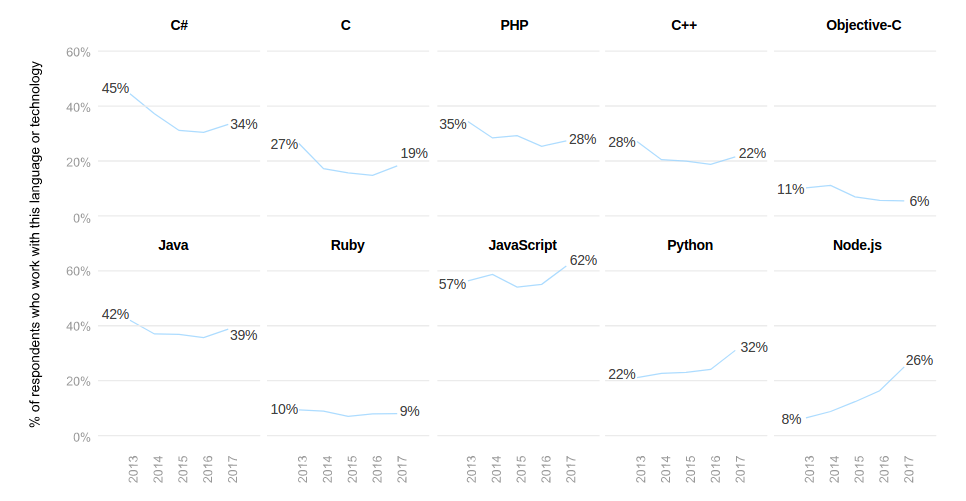
\includegraphics[scale=0.5]{survey17.png}}
	\caption{Developers survey for Stack Overflow website in 2017.}
	\label{survey17}
\end{figure}
Node.js~\cite{tilkov2010node} is an open-source, cross-platform JavaScript run-time environment for executing JavaScript code server-side. Node.js provides an event-driven architecture and a non-blocking I/O API designed to optimize application's throughput and scalability for real-time Web applications. It uses Google V8 JavaScript engine to execute code, and a large percentage of the basic modules are written in JavaScript. Node.js contains a built-in library to allow applications to act as a stand-alone Web server. The increasing popularity of Node.js in the last years can be seen in figure~\ref{survey17}.

\subsubsection{JSON}
\label{json}
In computing, JavaScript Object Notation or JSON~\cite{crockford2006application}, is an open-standard file format that uses human-readable text to transmit data objects consisting of attribute–value pairs and array data types (or any other serializable value). It is a very common data format used for asynchronous browser/server communication, including as a replacement for XML in some AJAX-style systems.
JSON is a language-independent data format. It was derived from JavaScript, but as of 2017 many programming languages include code to generate and parse JSON-format data. The official Internet media type for JSON is application/json. JSON filenames use the extension .json. JSON's basic data types are described below. \par
\paragraph{Number} A signed decimal number that may contain a fractional part and may use exponential E notation, but cannot include non-numbers like NaN. The format makes no distinction between integer and floating-point. JavaScript uses a double-precision floating-point format for all its numeric values, but other languages implementing JSON may encode numbers differently.
\paragraph{String} A string is a sequence of zero or more Unicode characters. Strings are delimited with double-quotation marks and support a backslash escaping syntax.
\paragraph{Boolean} Either of the values true or false.
\paragraph{Array} An ordered list of zero or more values, each of which may be of any type. Arrays use square bracket notation with elements being comma-separated.
\paragraph{Object} An unordered collection of name/value pairs where the names (also called keys) are strings. Since objects are intended to represent associative arrays, it is recommended, though not required, that each key is unique within an object. Objects are delimited with curly brackets and use commas to separate each pair, while within each pair the colon ':' character separates the key or name from its value.
\paragraph{null} An empty value, using the word null.

\subsubsection{Ajax}
\label{ajax}
\begin{figure}
	\centerline{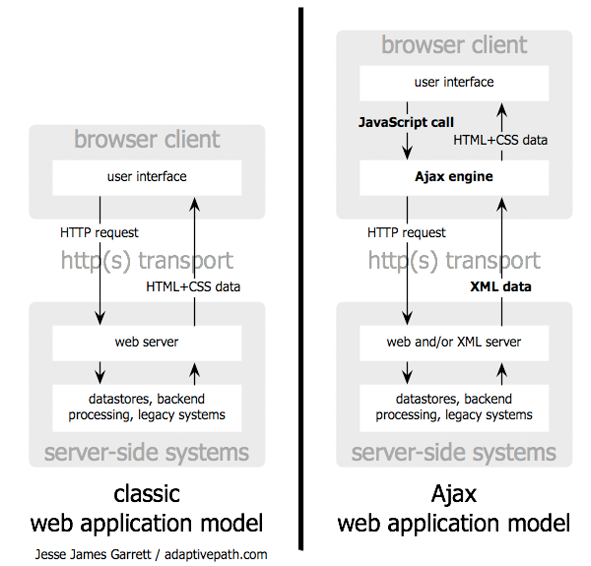
\includegraphics[scale=0.7]{ajax.png}}
	\caption{The traditional model for web applications (left) compared to the Ajax model (right)}
	\label{ajaxPNG}
\end{figure}
Ajax (short for "asynchronous JavaScript and XML")~\cite{garrett2005ajax} is a set of Web development techniques using many Web technologies on the client side to create asynchronous Web applications. With Ajax, Web applications can send data to and retrieve from a server asynchronously (in the background) without interfering with the display and behavior of the existing page. By decoupling the data interchange layer from the presentation layer, Ajax allows for Web pages, and by extension Web applications, to change content dynamically without the need to reload the entire page. In practice, modern implementations commonly substitute JSON for XML due to the advantages of being native to JavaScript.\par
Ajax is not a single technology, but rather a group of technologies. HTML and CSS can be used in combination to mark up and style information. The DOM is accessed with JavaScript to dynamically display – and allow the user to interact with – the information presented. JavaScript and the XMLHttpRequest object provide a method for exchanging data asynchronously between browser and server to avoid full page reloads.\par 
The term Ajax has come to represent a broad group of Web technologies that can be used to implement a Web application that communicates with a server in the background, without interfering with the current state of the page, such as HTML, CSS, DOM, XMLHttpRequest etc. The conventional model for a Web Application versus an application using Ajax can be seen in figure~\ref{ajaxPNG}.

\subsubsection{Node Package Manager}
Npm~\cite{schlueternode} is a package manager for the JavaScript programming language. It is the default package manager for the JavaScript runtime environment Node.js. It consists of a command line client, also called npm, and an online database of public packages called the npm registry. The registry is accessed via the client, and the available packages can be browsed and searched via the npm website. Npm is included as a recommended feature in Node.js installer. Npm consists of a command line client that interacts with a remote registry. It allows users to consume and distribute JavaScript modules that are available on the registry. Packages on the registry are in CommonJS format and include a metadata file in JSON format.

\subsection{NoSQL Database}
A NoSQL (originally referring to "non SQL" or "non-relational") database provides a mechanism for storage and retrieval of data that is modeled in means other than the tabular relations used in relational databases. NoSQL databases are increasingly used in big data and real-time web applications. Motivations for this approach include: simplicity of design, simpler "horizontal" scaling to clusters of machines (which is a problem for relational databases), and finer control over availability. The data structures used by NoSQL databases (e.g. key-value, wide column, graph, or document) are different from those used by default in relational databases, making some operations faster in NoSQL. The particular suitability of a given NoSQL database depends on the problem it must solve. Sometimes the data structures used by NoSQL databases are also viewed as "more flexible" than relational database tables.

\subsubsection{MongoDB}
MongoDB is a free and open-source cross-platform document-oriented database program. Instead of using tables and rows as in relational databases, MongoDB is built on an architecture of collections and documents, meaning fields can vary from document to document and data structure can be changed over time. Documents comprise sets of key-value pairs and are the basic unit of data in MongoDB. Collections contain sets of documents and function as the equivalent of relational database tables. \par 
	Like other NoSQL databases, MongoDB supports dynamic schema design, allowing the documents in a collection to have different fields and structures. The database uses a document storage and data interchange format called BSON, which provides a binary representation of JSON-like documents.



%\include{Chapters/Chapter4} 
%\include{Chapters/Chapter5} 

%----------------------------------------------------------------------------------------
%	BIBLIOGRAPHY
%----------------------------------------------------------------------------------------

\printbibliography[heading=bibintoc]

%----------------------------------------------------------------------------------------

\end{document}  
